\let\negmedspace\undefined
\let\negthickspace\undefined
\documentclass[journal]{IEEEtran}
\usepackage[a5paper, margin=10mm, onecolumn]{geometry}
%\usepackage{lmodern} % Ensure lmodern is loaded for pdflatex
\usepackage{tfrupee} % Include tfrupee package

\setlength{\headheight}{1cm} % Set the height of the header box
\setlength{\headsep}{0mm}     % Set the distance between the header box and the top of the text

\usepackage{gvv-book}
\usepackage{gvv}
\usepackage{cite}
\usepackage{amsmath,amssymb,amsfonts,amsthm}
\usepackage{algorithmic}
\usepackage{graphicx}
\usepackage{textcomp}
\usepackage{xcolor}
\usepackage{txfonts}
\usepackage{listings}
\usepackage{enumitem}
\usepackage{mathtools}
\usepackage{gensymb}
\usepackage{comment}
\usepackage[breaklinks=true]{hyperref}
\usepackage{tkz-euclide} 
\usepackage{listings}
% \usepackage{gvv}                                        
\def\inputGnumericTable{}                                 
\usepackage[latin1]{inputenc}                                
\usepackage{color}                                            
\usepackage{array}                                            
\usepackage{longtable}                                       
\usepackage{calc}                                             
\usepackage{multirow}                                         
\usepackage{hhline}                                           
\usepackage{ifthen}                                           
\usepackage{lscape}
\begin{document}

\bibliographystyle{IEEEtran}
\vspace{3cm}

\title{5.4.23}
\author{EE25btech11028 - J.Navya sri}
% \maketitle
% \newpage
% \bigskip
{\let\newpage\relax\maketitle}


\textbf{Question:} \\
Using elementary transformations, find the inverse of the following matrix:
\[
A = \myvec{2 & -3 \\ -1 & 2}
\]



\textbf{Soultion:}
We want to find the inverse of the matrix
\[
A = \myvec{2 & -3 \\ -1 & 2}.
\]

\textbf{Step 1: Assume the inverse matrix}

Let
\begin{equation}
A^{-1} = \myvec{x & y \\ z & w}
\end{equation}

By definition of inverse, we have
\begin{equation}
A A^{-1} = I = \myvec{1 & 0 \\ 0 & 1}
\end{equation}

\textbf{Step 2: Multiply the matrices}

\begin{equation}
\myvec{2 & -3 \\ -1 & 2} \myvec{x & y \\ z & w} =
\myvec{2x - 3z & 2y - 3w \\ -x + 2z & -y + 2w}
\end{equation}

\begin{equation}
\myvec{2x - 3z & 2y - 3w \\ -x + 2z & -y + 2w} = 
\myvec{1 & 0 \\ 0 & 1}
\end{equation}

From this multiplication, we get the following system of equations:

\begin{equation}
2x - 3z = 1
\end{equation}

\begin{equation}
2y - 3w = 0
\end{equation}

\begin{equation}
-x + 2z = 0
\end{equation}

\begin{equation}
-y + 2w = 1
\end{equation}

\textbf{Step 3: Solve the equations}

From equation (7):
\begin{equation}
-x + 2z = 0 \Rightarrow x = 2z
\end{equation}

Substitute into equation (5):
\begin{equation}
2(2z) - 3z = 1 \Rightarrow 4z - 3z = 1 \Rightarrow z = 1
\end{equation}

Then,
\begin{equation}
x = 2z = 2
\end{equation}

From equation (8):
\begin{equation}
-y + 2w = 1 \Rightarrow y = 2w - 1
\end{equation}

Substitute into equation (6):
\begin{equation}
2(2w - 1) - 3w = 0 \Rightarrow 4w - 2 - 3w = 0 \Rightarrow w = 2
\end{equation}

Then,
\begin{equation}
y = 2w - 1 = 3
\end{equation}

\textbf{Step 4: Write the inverse matrix}

\begin{equation}
A^{-1} = \myvec{2 & 3 \\ 1 & 2}
\end{equation}

\textbf{Graph presentation:}
\begin{figure}[H]
\begin{center}
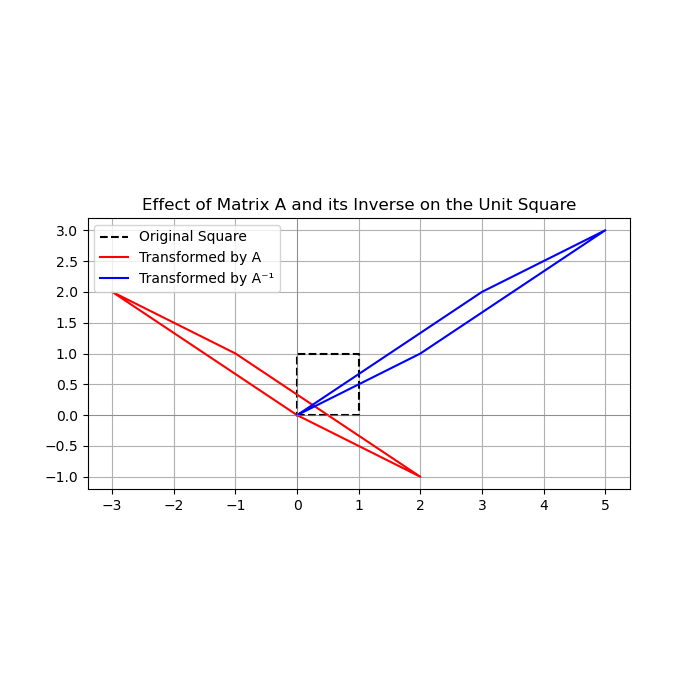
\includegraphics[width=0.6\columnwidth]{Figs/fig11.png}
\end{center}
\caption{}
\label{fig:Fig}
\end{figure}
\end{document}

